\documentclass[11pt,a4paper]{article}
\usepackage[margin=2.5cm]{geometry}
\usepackage{graphicx}
\usepackage{caption}
\usepackage{subcaption}
\usepackage{hyperref}
\usepackage{amsmath}
\hypersetup{colorlinks=true, urlcolor=blue, linkcolor=blue}
\usepackage{float}
\usepackage{wasysym}
\usepackage[utf8]{inputenc}
\DeclareUnicodeCharacter{2300}{\diameter}   % 2300 is the hex code of ⌀



\title{\textbf{PSM Protech Feasibility Study}\\Technical Documentation}
\author{Internal Project Documentation \\ PSM Protech}
\date{\today}


\begin{document}

\maketitle
\thispagestyle{empty}
\begin{center}
\newpage
\textbf{Abstract}
\end{center}
\noindent
This document provides a comprehensive technical overview of the PSM Protech Feasibility Study project. The project aims to automate the extraction and analysis of geometric tolerances from engineering drawings using computer vision and machine learning techniques. It is intended to onboard new team members by explaining the project context, goals, methodology, system architecture, tools, models, data, constraints, current progress, results, and planned next steps. The document is structured as a reference guide for internal use, designed to be extended in future project phases.

\vfill
\newpage
\tableofcontents
\newpage

\section{Initial Situation}
PSM Protech is a leading manufacturer of high-precision mechanical components and assemblies serving the aerospace, medical, and industrial sectors. The company specializes in tight tolerance CNC machining, rapid prototyping, and comprehensive quality assurance to deliver complex parts with consistent accuracy and reliability.

Mechanical engineering drawings are detailed technical plans that specify dimensions and tolerances for manufactured parts. Each drawing can contain hundreds of annotations that define the allowable variation in part geometry (known as GD\&T -- \emph{Geometric Dimensioning and Tolerancing} specifications). Traditionally, engineers at PSM Protech manually review these drawings to assess feasibility of production, a process that is time-consuming (2 weeks) and prone to human error. For example, Figure~\ref{fig:example_drawing} shows an engineering drawing of a mechanical part with numerous GD\&T callouts (tolerance symbols and values referencing datums). Manually checking up to 500 individual tolerance values in such a drawing, often across multiple design revisions, is tedious and carries the risk of overlooking critical requirements.

\begin{figure}[h!]
\centering
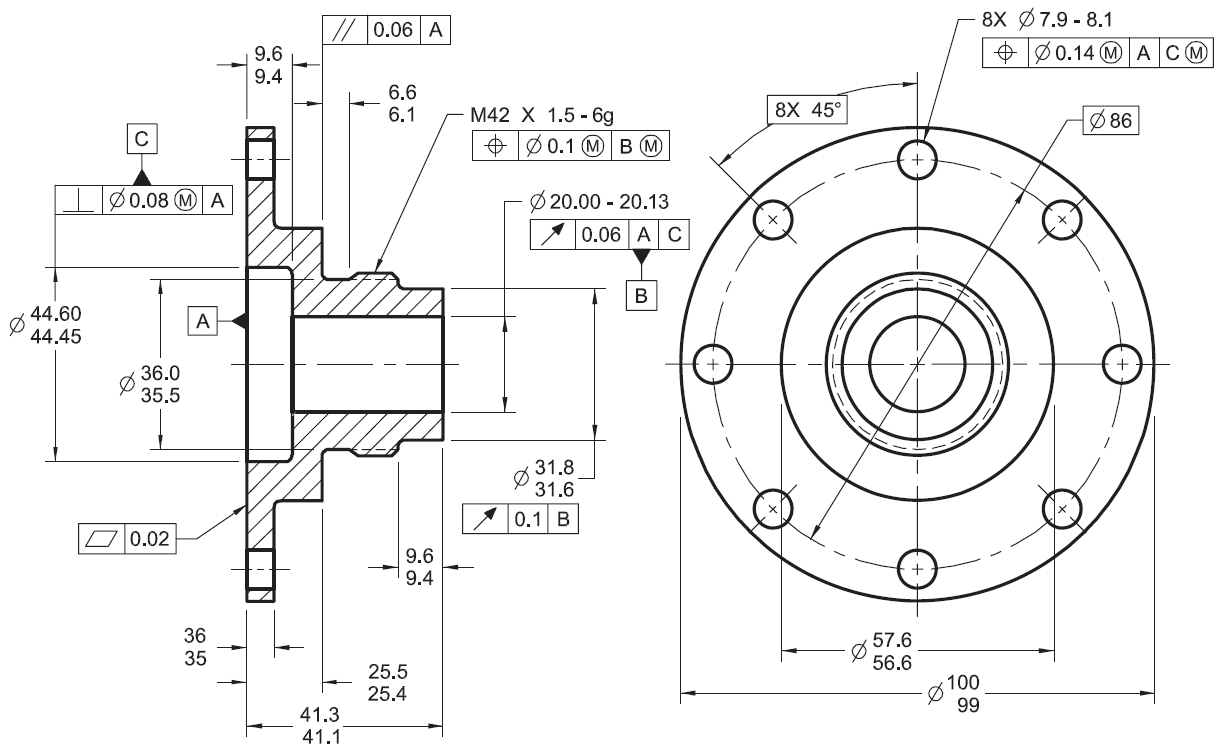
\includegraphics[width=\textwidth]{GDD-Drawing-Example.png}
\caption{Example of an engineering drawing with multiple geometric tolerances (GD\&T) annotations. Such drawings contain numerous dimensions and tolerance callouts (in feature control frames) that must be verified for feasibility.}
\label{fig:example_drawing}
\end{figure}

Given this context, PSM Protech initiated a feasibility study to investigate whether computer vision and AI techniques can automate the evaluation of these drawings. By automatically extracting tolerance information and identifying critical values, the company aims to reduce the workload on engineers and minimize the chance of missing important constraints. This project is part of a broader push towards digital transformation in the engineering review process.
\begin{figure}[h!]
\centering
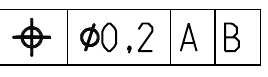
\includegraphics[width=0.2\textwidth]{45.png}
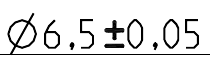
\includegraphics[width=0.2\textwidth]{46.png}
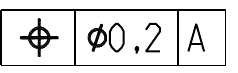
\includegraphics[width=0.2\textwidth]{47.png}
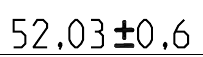
\includegraphics[width=0.2\textwidth]{60.png}
\label{fig:1}
\end{figure}

\section*{Related Work}
This section reviews existing approaches and tools for extracting structured data from engineering and technical drawings, highlighting methods relevant to our project.

\subsection*{Academic Approaches}
\begin{itemize}
  \item \textbf{Hybrid Deep-Learning for Structured Extraction}: Zheng et al. integrate an oriented
    bounding-box detector (YOLOv11) with a document-understanding transformer (Donut) to
    extract and parse key annotation categories (e.g., GD\&T, tolerances, materials).
  \item \textbf{Tolerance Information Extraction}: Xu et al. (2024) combine image-processing pipelines
    with a CNN-based recognizer to extract tolerance data from mechanical drawings.
  \item \textbf{eDOCr2 Framework}: The eDOCr2 framework (MDPI, 2023) fuses conventional OCR with
    tailored image-processing to pull structured data (dimensions, notes, tolerances) from 2D
    technical drawings.
\end{itemize}

\subsection*{Open-Source and Commercial Solutions}
\begin{itemize}
  \item \textbf{engineering-drawing-extractor (GitHub)}: Bakkopi’s project automates region isolation
    and OCR to capture drawing metadata (numbers, titles, authors).
  \item \textbf{Werk24 API}: A commercial AI service offering specialized extraction of structured
    data (including tolerances and BOM) from technical drawings.
  \item \textbf{Infrrd and Markovate AI Blueprint Reader}: Platforms combining machine learning,
    OCR, and workflow automation to streamline blueprint processing in preconstruction planning.
\end{itemize}


\section{Goal}
The primary goal of the \textbf{PSM Protech Feasibility Study} project is to develop an automated system that can interpret mechanical drawings and extract key tolerance specifications for further analysis. In particular, the system should:
\begin{itemize}
  \item \textbf{Automatically identify geometric tolerance annotations} (GD\&T feature control frames and related text) in a given drawing.
  \item \textbf{Classify the type of each tolerance} (e.g., flatness, cylindricity, etc.) to understand what kind of constraint it represents.
  \item \textbf{Extract the numerical tolerance values} associated with each annotation with high precision.
  \item \textbf{Aggregate and present the extracted data} in a structured format for review, allowing automatic check against feasibility criteria.
  \item \textbf{Highlight critical tolerances or changes} between drawing revisions, so engineers can quickly focus on potential problem areas.
\end{itemize}

Ultimately, achieving these goals would mean that when a new part drawing or an updated revision is received, the system could quickly parse it and produce an excel report of all tolerance requirements. This would greatly speed up the feasibility assessment phase and allow engineers to concentrate on addressing the critical issues rather than manually transcribing the data.

\begin{center}
  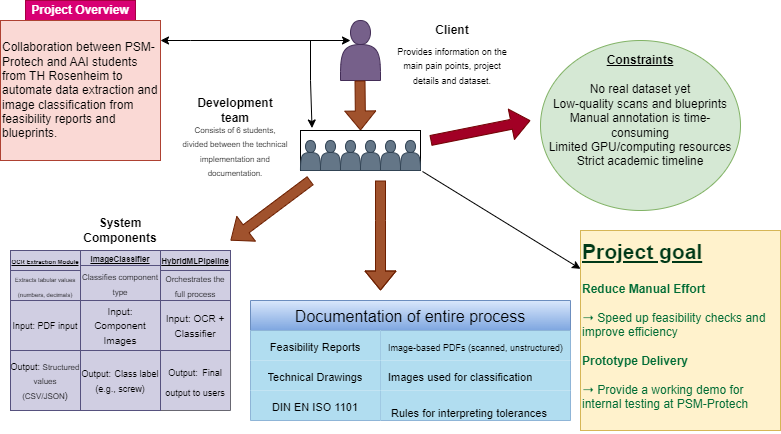
\includegraphics[width=\textwidth]{Rich-Picure.drawio.png}\\[5mm]
  % “5mm” of extra vertical space before the next line
    Rich Picture
\end{center}

\section{Methodology}
To accomplish project goals, our approach combines computer vision, deep learning, and optical character recognition (OCR) in a hybrid pipeline. The methodology has been structured in iterative phases, focusing on building and validating individual models, which will later be integrated. The core idea is to let machine learning handle visual recognition tasks (such as identifying symbol types) and use OCR techniques to read text (numerical values), playing to the strengths of each technique. 

At a high level, the methodology is as follows:
\begin{enumerate}
    \item \textbf{Data Preprocessing}: Annotating each image based on what the model expects for training. Detailed explanation can be found in (Section 6).
    \item \textbf{Tolerance Models}: We employ four models—\texttt{falcon\_r1}, \texttt{falcon\_r2}, \texttt{falcon\_r3}, and \texttt{falcon\_r4}. We have different models for different purposes ranging from cropping to classification. We train a deep learning model to recognize the type of tolerance from an image of its symbol (for example, distinguishing a flatness symbol from a cylindricity symbol). We fine-tuned pre-trained YOLOv8 and subsequently YOLOv11 convolutional neural networks in classification mode on our dataset of labeled tolerance symbol images. For more information, refer to Section~6.
    \item \textbf{Containerization}: We plan to containerize the system using Docker. Additionally, we plan the combination of the classification model and OCR extraction into a single end-to-end system. In a complete workflow, the system would scan an entire drawing, detect regions that contain tolerance information (e.g., using object detection techniques), classify each detected region's tolerance type, and apply OCR to extract the corresponding value(s).
    \item \textbf{Iteration and Validation}: Evaluate the performance of each component on test images, identify weaknesses, and improve the methodology. This includes refining the synthetic data generation, tuning model hyperparameters, and improving image preprocessing steps for OCR. Future iterations will incorporate real-world drawing data to validate the approach in practice.
\end{enumerate}

In summary, our methodology is a hybrid approach that blends machine learning for pattern recognition (tolerance symbols classification) with OCR techniques for reading text. By breaking down the problem into these components, we address each challenge (visual classification vs. text reading) with an appropriate tool, and then assemble the pieces into a cohesive pipeline.

\section{System Architecture}
The system architecture for the proposed solution can be viewed as a pipeline of modular components, each responsible for a specific function in the overall process of tolerance extraction. illustrates the conceptual flow of data through the system, from input drawing to output report. The main components of the architecture include:
\begin{figure}[h!]
\centering
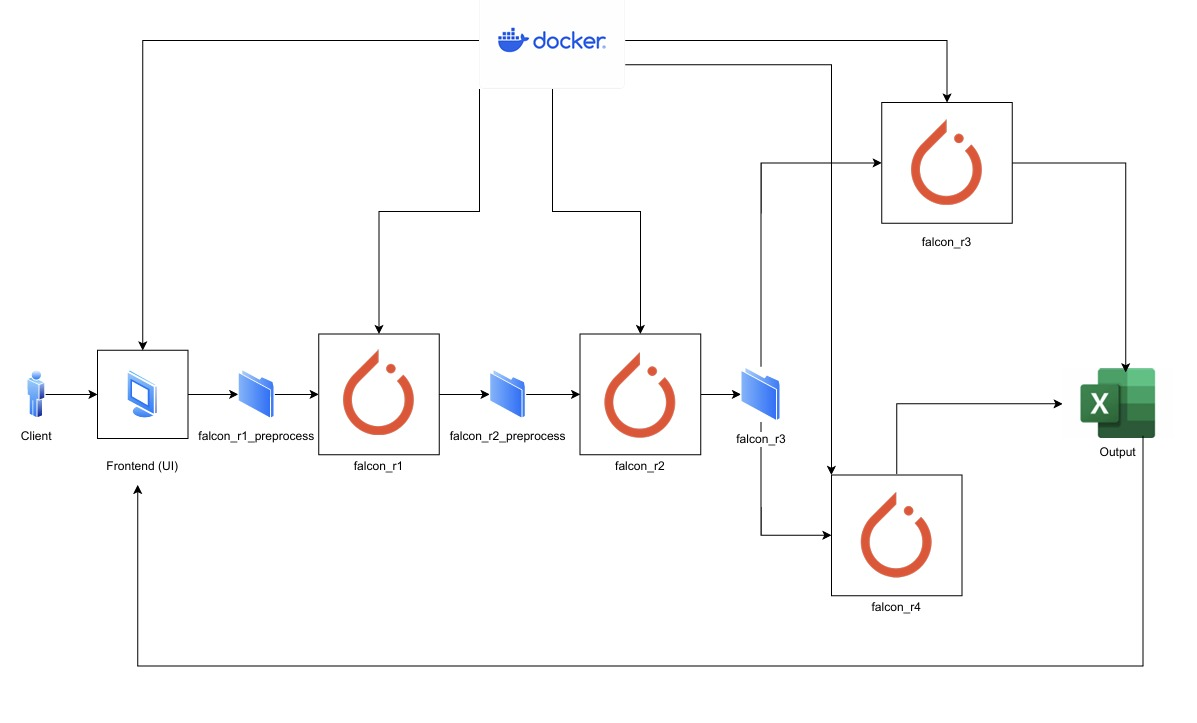
\includegraphics[width=0.9\textwidth]{System Archi.png}
\caption{System architecture overview showing the flow from input drawing to extracted tolerance data. (This is a placeholder for a high-level flowchart or diagram.)}
\label{fig:Arch_Flow}
\end{figure}

\begin{itemize}
  \item \textbf{Input Module}: Accepts the engineering drawing input. In the current feasibility study, this is either a PDF file or image files (e.g., scanned drawings or synthesized images). Preprocessing may be applied here to improve image quality (e.g., converting CAD PDFs to images, grayscaling, etc.).
  \item \textbf{Region Detection (Planned)}: In a full implementation, an object detection model (such as a YOLOv8 object detector) would scan the drawing to locate regions that contain tolerance information (feature control frames, dimensions, notes). \emph{This step is planned for a future iteration; in the current phase, we assume the regions of interest are provided or use prepared images that isolate the tolerance annotations.}
  \begin{figure}[h!]
  \centering
  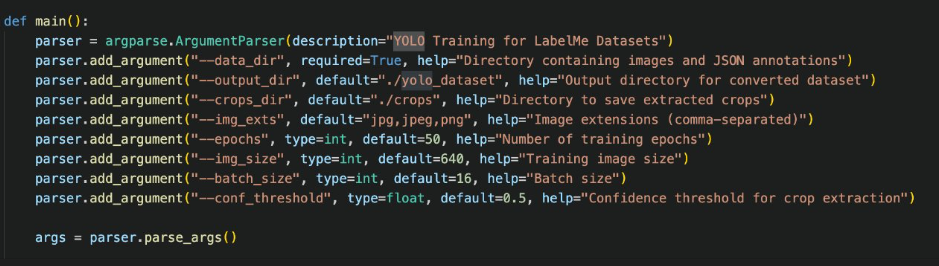
\includegraphics[width=0.9\textwidth]{Segment_Model.png}
  \caption{Segment Model}
  \end{figure}
  \item \textbf{Tolerance Classification Module}: Each identified region or annotation image is passed to a classification model which determines the type of tolerance symbol present. This module uses the trained YOLOv8 classification network. For instance, it will output labels like “flatness” or “cylindricity” for the given image region.
\begin{figure}[h!]
\centering
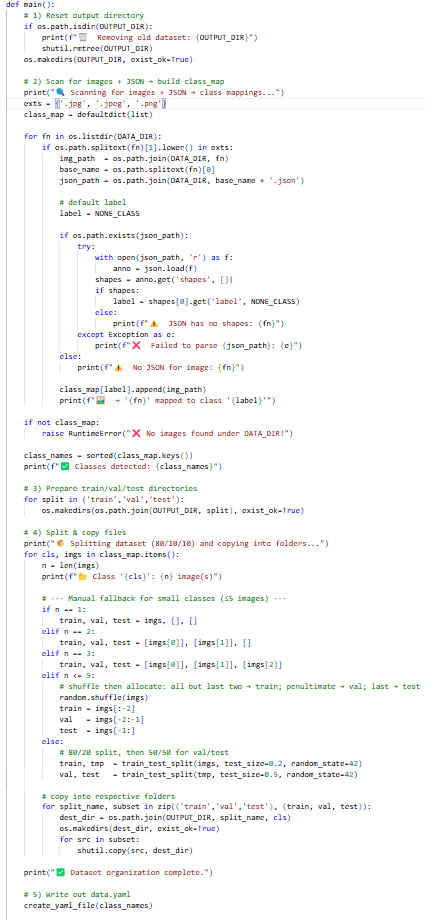
\includegraphics[width=0.9\textwidth]{Classification_Model.png}
\caption{Classification Model}
\end{figure}
  \item \textbf{OCR Extraction Module}: Parallel to (or following) classification, the system extracts the numerical tolerance values from the annotation. This is done by the OCR pipeline which may involve converting the region to PDF (to leverage any embedded text via parsing) and/or directly applying image OCR. The module returns the numeric value(s) associated with that tolerance. For example, it might read a value like “0.05” from the image, possibly also capturing any modifier (though currently we focus on the numeric magnitude).

  \item \textbf{Data Aggregation and Output}: The results from classification and OCR are combined. Each tolerance annotation thus yields a structured record (e.g., \{type: flatness, value: 0.05, units: mm, referenced datums: A, B\}). These records are then compiled into an output format such as a CSV file or a summarized report. The output can be reviewed by engineers or fed into further analysis tools to check feasibility criteria. In our prototype, the OCR pipeline writes the results to a CSV file for simplicity.
    \begin{figure}[h!]
  \centering
  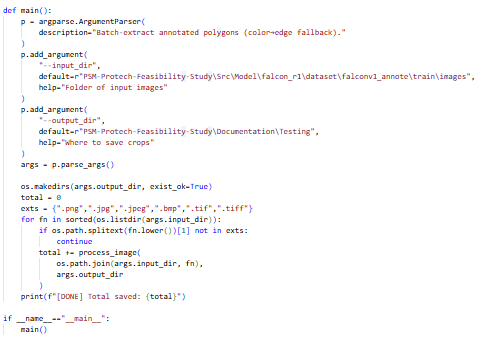
\includegraphics[width=0.9\textwidth]{OCR Extraction.png}
  \caption{OCR Extraction}
  \end{figure}
\end{itemize}

The above architecture is modular: the classification and OCR extraction components operate independently and can be improved or replaced without affecting the other, as long as they adhere to the defined interface (input image, output label or text). Currently, these components are implemented as separate scripts, and integration is done manually by feeding the output of one into the other. As the project progresses, these will be unified into a single pipeline. Notably, in this feasibility stage, we have deliberately separated the concerns of “what is the tolerance type?” and “what is the tolerance value?”, but in a production system they would work in tandem on each detected annotation region.

\section{Tools \& Frameworks Used}
Throughout the project, we have utilized a range of software tools, libraries, and frameworks to implement the solution. Below is a summary of the key technologies and their roles:

\begin{itemize}
  \item \textbf{Python 3}: The primary programming language used for all development in this project. Python was chosen for its extensive ecosystem of libraries in computer vision and machine learning, as well as its ease of rapid prototyping.
  \item \textbf{Ultralytics YOLOv8}: A cutting-edge deep learning model framework specialized for object detection and classification. We use the YOLOv8 implementation (via the \verb|ultralytics| Python package) in \textbf{classification mode} to train a model for tolerance symbol recognition. YOLOv8 provides pre-trained weights and an easy training API, which significantly accelerated model development.
  \item \textbf{OpenCV} (cv2) and \textbf{PIL (Python Imaging Library)}: Used for image processing tasks such as reading images, converting color spaces, resizing, and cropping. OpenCV in particular is used in the OCR pipeline for preprocessing images (grayscaling, blurring, thresholding) to improve OCR results.
  \item \textbf{PyTesseract} (Tesseract OCR engine): An open-source OCR engine used to extract text from images. We integrate PyTesseract for reading the numeric tolerance values from image regions. Tesseract is configured to be numeric-only (digits and decimal points) in our pipeline to reduce errors from unrelated text.
  \item \textbf{Camelot}: A Python library for PDF table extraction. Camelot is employed in the pipeline to attempt reading tolerance values from PDFs (if the drawing data is vectorized or if an annotation can be interpreted as a table). If the tolerance information is structured in a table in a PDF, Camelot can directly extract cell contents, which is faster and potentially more accurate than OCR. In our use case, Camelot is run in \emph{stream} mode, which looks for line structures in the PDF to parse tables.
  \item \textbf{pandas}: A data analysis library used here for assembling the final results into a tabular format (DataFrame) and writing output to CSV. After processing all images, we use pandas to create a table of extracted values for easy viewing and further analysis.
  \item \textbf{scikit-learn}: Specifically, we use the \verb|train_test_split| utility to split the synthetic dataset into training and validation subsets for model training. This ensures we can evaluate the classification model’s performance on unseen data.
  \item \textbf{Logging}: Python’s built-in \verb|logging| module is used to record informative messages during execution of the pipelines. This includes logging steps of the process and any warnings or errors (e.g., if OCR fails to find a number in a region).
  \item \textbf{Miscellaneous}: Other standard libraries include \verb|NumPy| (for numerical operations and array manipulation) and \verb|pathlib| for file path management. These help with handling image data and filesystem interactions in a platform-independent way.
\end{itemize}

By leveraging these frameworks and libraries, we avoided reinventing the wheel for common tasks and instead focused on the project-specific logic. The combination of YOLOv8 for classification and Tesseract for OCR, in particular, allowed us to implement a solution using state-of-the-art tools with relatively little custom code.

\section{Model Explanations}
This section provides details on the two main components of the project: the tolerance classification model and the OCR extraction pipeline. For each, we explain how the model or algorithm works and summarize the implementation (referring to the code in \verb|classification.py| and \verb|ocr_pipeline.py| respectively).

\subsection{Tolerance Classification Model (YOLOv8-CLS)}
The tolerance classification model is based on the YOLOv8 architecture, configured for single-image classification. Instead of detecting objects in a large image, we feed it cropped images of individual tolerance annotations (mostly the GD\&T symbol and its frame) and train it to output the class of tolerance.

\paragraph{Model Architecture:} YOLOv8 in classification mode is a convolutional neural network (CNN) that has been pre-trained (on ImageNet) to recognize generic image features. We fine-tuned the model on our specific classes of interest. Each class corresponds to a type of geometric tolerance. In our synthetic dataset, examples of classes include \texttt{flatness}, \texttt{cylindricity}, and potentially others such as straightness or perpendicularity (depending on the range of symbols we included). The model’s last layer produces an output probability for each class, and we take the highest probability as the predicted class for an input image.

\paragraph{Training Procedure:} The training process for the classifier is encapsulated in the \verb|classification.py| script. The key steps are:
\begin{enumerate}
    \item \textbf{Dataset Parsing}: The script scans the dataset directory (containing our annotated synthetic images). It automatically infers class names by looking at the filename prefixes (each image file is named with its class, e.g., \verb|form_flatness.png|, \verb|form_cylindricity.png|, etc.). All images are grouped by class label.
    \item \textbf{Train-Validation Split}: The gathered images for each class are split into a training set and a validation set (80\% train, 20\% val). This ensures that we can evaluate the model’s generalization on images it wasn’t trained on. The script creates a directory structure expected by YOLO (separate \verb|train/| and \verb|val/| folders, each containing subfolders for each class with the respective images).
    \item \textbf{Model Training}: We load a YOLOv8 classification model with pre-trained weights (in our case, we specified the \verb|yolov8l-cls.pt| model, which is a large variant for classification). The training is then executed via the Ultralytics API call \verb|model.train(...)|, specifying parameters such as number of epochs (we used 10 epochs as an initial training period), image size (224 pixels), batch size (32), and the device (using GPU if available). The model automatically learns to distinguish the classes by adjusting its internal weights on the training images. During training, we can see progress metrics such as training/validation accuracy and loss.
    \item \textbf{Model Saving}: After training, the best-performing model weights (based on validation loss) are saved to disk (the script will output the path, typically \texttt{}|runs/classify/train/weights/best.pt| or similar). This saved model can later be loaded for inference on new images.
\end{enumerate}

In essence, the classification model learns to recognize different GD\&T symbols. For example, the flatness symbol (a parallelogram shape) looks very different from the cylindricity symbol (which appears as a circle or cylinder icon). By training on many examples of each, the CNN can reliably identify the type when shown a new instance. This classifier will be crucial when processing a full drawing: it will allow the system to know what kind of tolerance each detected annotation represents, which is necessary for any further reasoning (like understanding which tolerances are critical, or grouping similar types, etc.).

\paragraph{Usage:} Once trained, using the model is straightforward. An input image (say, a cropped region from a drawing focusing on a tolerance frame) is passed to the model’s predict function, and it returns the predicted class label (and confidence). For instance, given an image of a symbol like in Figure~\ref{fig:synthetic_samples} (left), the model should output “flatness.” 

% Insert figure of synthetic samples (flatness and cylindricity)
\begin{figure}[h!]
\centering
\begin{subfigure}{0.45\textwidth}
  \centering
  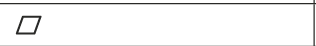
\includegraphics[width=\textwidth, trim=0 0 0 0, clip]{form_flatness.png}
  \caption{Flatness tolerance symbol}
\end{subfigure}\hfill
\begin{subfigure}{0.45\textwidth}
  \centering
  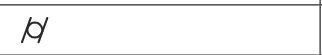
\includegraphics[width=\textwidth, trim=0 0 0 0, clip]{form_cylindricity.png}
  \caption{Cylindricity tolerance symbol}
\end{subfigure}
\caption{Examples of synthetic training images for the classification model, showing GD\&T symbols: (a) flatness and (b) cylindricity. These simple images consist of the geometric symbol in a frame, similar to how they appear on drawings. The classification model learns to differentiate such symbols.}
\label{fig:synthetic_samples}
\end{figure}

\subsection{OCR Extraction Pipeline}
The OCR extraction pipeline is implemented in the \verb|ocr_pipeline.py| script. Its purpose is to extract the numerical tolerance values (and potentially related information) from the images. This pipeline is described as “hybrid” because it uses two approaches: first, an attempt to parse any structured table data using Camelot (which works if the input PDF contains machine-readable text or tables), and second, a fallback to optical character recognition using Tesseract on image data if Camelot cannot retrieve the information.

Here’s a breakdown of how the OCR pipeline works:

\paragraph{Pipeline Steps:} The main routine (\verb|TableOCRExtractor.run()| method) processes each image in the dataset sequentially:
\begin{enumerate}
    \item \textbf{Image to PDF Conversion}: For each image file, we convert the image into a one-page PDF file. This is done because Camelot expects a PDF input. Using \verb|PIL|, the image (which might be a snippet of a drawing containing a tolerance specification) is embedded into a PDF page.
    \item \textbf{Table Parsing with Camelot}: We call Camelot’s \verb|read_pdf| on the generated PDF, using the "stream" flavor (which looks for lines in the page to delineate table cells). If the tolerance annotation is structured like a small table or if the PDF contains actual text, Camelot may detect a table and return a DataFrame of the cell contents. The script checks if any tables were found. If yes, it extracts the relevant cells (in our case, we expect the tolerance values to be in specific columns of the table). For instance, if the table has columns for the tolerance symbol, nominal value, and tolerance value, the pipeline knows to read, say, the second and third columns as the output.
    \item \textbf{PDF to Image Rendering (fallback path)}: If Camelot fails to find a table (which is common if the PDF page is essentially just an embedded image with no real text), the pipeline falls back to image-based OCR. We then render the PDF page back into an image (this may seem roundabout, but it ensures we have a consistent image format, e.g., a high-DPI raster image of the annotation). Using \verb|pdf2image|, we get a PIL image of the page.
    \item \textbf{Crop Regions of Interest}: We assume a known layout for the tolerance annotation: typically, there might be multiple columns of text. In our synthetic data, for example, we designed the image such that the second column contains one number (perhaps a requirement or measured value) and the third column contains another number (perhaps a tolerance limit). The pipeline crops the rendered image into two sub-images: column 2 and column 3. (The cropping coordinates are determined as fractions of the total width: e.g., 20\% to 60\% of width for the first number, 60\% to 98\% for the second number, based on how we formatted the synthetic data.)
    \item \textbf{Image Preprocessing}: Each cropped region image is then preprocessed to improve OCR accuracy. Preprocessing steps include converting to grayscale, applying a slight Gaussian blur (to reduce noise), using Otsu’s thresholding to get a binary image (black text on white background), inverting the image (to have black text on white if needed), and scaling it up (magnifying by 2x) to help Tesseract read small text.
    \item \textbf{OCR with Tesseract}: The preprocessed image of each region (column) is fed into PyTesseract. We configure Tesseract with a character whitelist of digits and the decimal point, since we expect only numeric values. Tesseract returns any text it can read. We then use a regex (regular expression) to find a numeric pattern in that text (e.g., something matching a decimal number format). If a number is found, we record it as the value for that region.
    \item \textbf{Result Recording}: For each original image, if we successfully extracted values (either via Camelot or OCR), we append a result entry to a list. Each result is typically a dictionary or similar structure containing the source image name and the extracted column2 and column3 values.
\end{enumerate}

After processing all images, the pipeline uses \verb|pandas| to save the results list as a CSV file (named \verb|extracted_numbers.csv|). Each row in this CSV corresponds to an input image (identified by name) and contains the numbers that were extracted from that image.

\paragraph{Example:} Suppose an input image contains a tolerance annotation for flatness, with a value of 0.02 mm. If this image were structured such that the tolerance symbol is in one column and the value "0.02" in the next column, the pipeline’s OCR would ideally output something like:
\[
\{\text{source\_image}: \text{"flatness\_example"},\; \text{col2}: 0.02,\; \text{col3}: \text{None}\} 
\]
(if only one number was present in col2 and no second number in col3). In another case, if an annotation had two numeric values (for instance, an upper and lower bound), both col2 and col3 would be filled.

\paragraph{Handling Failures:} The pipeline is designed to be robust to missing data: if a region’s OCR does not find any number, it logs a warning and continues. In our initial tests on synthetic images, the OCR step works reliably because the text is clear. However, in real-world scenarios, text could be skewed, smaller, or have background interference, which may require more advanced image processing (deskewing, using adaptive thresholding, etc.). We have the logging in place to analyze such cases later.

\paragraph{Integration with Classification:} It’s worth noting that currently the OCR pipeline does not explicitly use the classification result. In a fully integrated system, once a tolerance type is known from the classifier, we might use that information to decide how to interpret the numbers. For example, a positional tolerance might have two numbers (like diametrical tolerance zone, plus maybe datum references), whereas a flatness tolerance has a single value. Knowing the type could help validate that the correct number of values were extracted and possibly attach units (most linear tolerances in our context are in millimeters, but angle tolerances or other types might have different units). Such integration will be considered in future development. For now, the OCR pipeline simply attempts to extract any numeric values present in the annotation image.

\section{Datasets (Synthetic Data)}
Because obtaining a large number of real annotated engineering drawings was not feasible at the project’s start, we created a synthetic dataset to train and evaluate our models. The synthetic data serves to mimic the appearance of tolerance annotations one would find on real drawings, but in a controlled and reproducible way.

\section*{Alternative Approach}
Due to delays in receiving customer-provided blueprints, we adopted an alternative workflow to ensure continuous progress:

\begin{enumerate}
  \item \textbf{Synthetic Data Source:} We obtained sample drawings in the DIN file format containing demonstration gear diagrams.
  \item \textbf{Bounding-Box Extraction:} From these demonstration files, we programmatically extracted bounding boxes around parts and their associated annotation regions.
  \item \textbf{Model Prototyping:}
    \begin{itemize}
      \item \textbf{Classification Model:} Trained on synthetic crops of extracted symbols to assign them to predefined classes.
      \item \textbf{OCR Extraction Model:} Trained on synthetic text crops to recognize numeric values and tolerances.
    \end{itemize}
  \item \textbf{Preliminary Results:} Both models achieved near-perfect performance (100\% accuracy) on the synthetic dataset, validating our training pipeline.
  \item \textbf{Integration with Real Data:} Upon delivery of actual customer blueprints, we plan to fine-tune both models using real annotations to account for domain differences.
\end{enumerate}

\begin{figure}[h!]
  \centering
    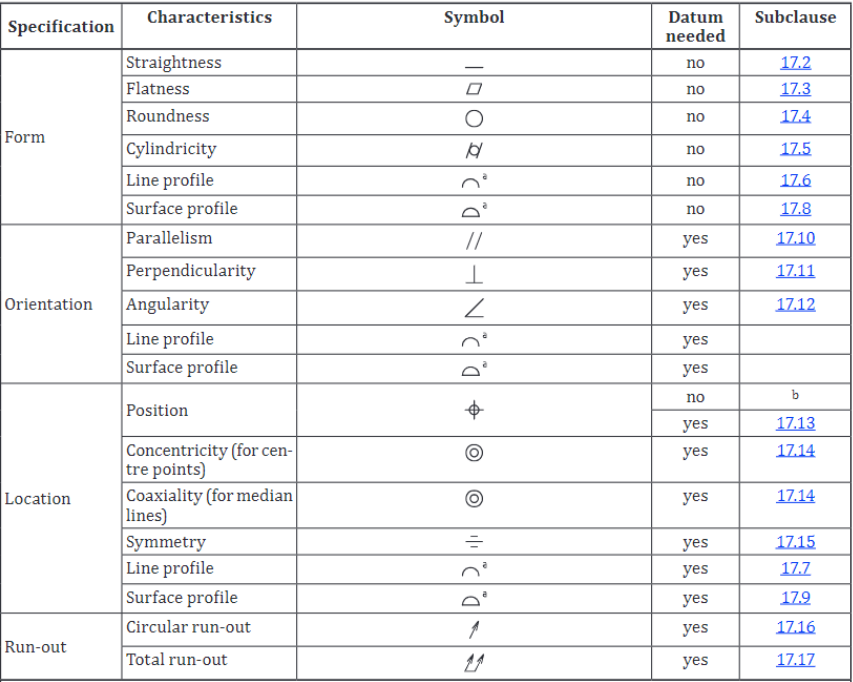
\includegraphics[width=\textwidth]{alternative_approach.png}%
  \caption{Main geometric tolerancing table used for synthetic data creation.}
  \label{fig:geom_tol}
\end{figure}

\section{Deliverables}
\begin{table}[H]
  \centering
  \begin{tabular}{p{0.45\textwidth} p{0.45\textwidth}}
    \textbf{Target Description} & \textbf{Success Criteria} \\
    Automate evaluation of mechanical drawings to reduce manual costs & Blueprint evaluations proceed without manual intervention, reducing overall review workload. \\
    Extract part diagrams from blueprints via large-scale cropping & The system reliably isolates and crops each part diagram from source blueprints for further processing. \\
    Identify critical tolerances and feasibility issues based on extracted data and predefined rules & Tolerance data and feasibility concerns are accurately highlighted according to the established rule set. \\
    Classify extracted symbols from cropped regions into their respective classes & Symbols detected within cropped regions are correctly assigned to their defined categories. \\
    Generate a comprehensive Excel sheet linking cropped drawings to their embedded information (symbols, values, tolerances) & The output spreadsheet lists every cropped diagram paired with its corresponding extracted data fields. \\
  \end{tabular}
  \caption{Overview of project deliverables with corresponding success criteria.}
  \label{tab:deliverables}
\end{table}


\subsection*{Dataset Size and Split}
In total, the synthetic dataset contains on the order of tens of images per class (for example, 20 flatness images and 20 cylindricity images, etc., resulting in perhaps ~100 images if five classes were considered). This is a relatively small dataset, but sufficient for a feasibility test given the simplicity of the images. The dataset was divided into training and validation sets for the classification model (as described earlier, 80/20 split). 

For OCR pipeline development, a portion of images (separate from those used in training the classifier) were used as test input to simulate the extraction process. In some cases, the same image could be used to both classify the symbol and then read the value.

\subsection*{Quality and Limitations of Synthetic Data}
While the synthetic data allowed us to get started, it has limitations. The images are generally cleaner and simpler than real drawing scans or PDFs. Real drawings might have noise, skew, multiple overlapping elements, or variations in how symbols and text are rendered (different line weights, CAD fonts, etc.). Therefore, the models trained on synthetic data may not directly translate to real data without further fine-tuning. Nonetheless, using synthetic data was a crucial first step to prove that our approach (the combination of classification and OCR) can work in principle. It provided quick feedback and validation of the algorithms in a controlled scenario.

In future work, we plan to incorporate real drawings (with ground-truth annotations done by experts) into the dataset to improve realism. The synthetic dataset can also be expanded with programmatically generated images (for example, using a script to draw random tolerance values and symbols) to increase quantity and diversity.

\section{Constraints}
During the development of this feasibility study, several constraints and challenges were identified. Understanding these constraints is important for interpreting the current results and planning the next steps:

\begin{itemize}
  \item \textbf{Limited Real Data:} A major constraint was the scarcity of real-world training data. We did not have access to a large repository of annotated engineering drawings to directly train our models. This led to the reliance on synthetic data, which, while useful, may not capture the full complexity of real drawings.
  \item \textbf{Variety of Tolerance Types:} Geometric tolerances encompass a wide range of symbols and notations (flatness, straightness, roundness, parallelism, perpendicularity, angularity, position, concentricity, etc.). In this initial phase we only tackled a small subset. Extending to all types (and combinations, e.g., a position tolerance with certain material condition symbols) increases complexity.
  \item \textbf{Complex Layouts:} On a full drawing, tolerance information can appear in different contexts: in feature control frames next to the features, or in tabular form (like a tolerance table or notes section). Our current pipeline handles isolated annotation images but not the full-page layout problem. The detection of where these annotations are on a large drawing is an unsolved part (to be addressed with object detection).
  \item \textbf{OCR Accuracy:} OCR can be error-prone, especially with small font sizes or non-standard fonts. Tesseract might misread characters (e.g., interpreting “0.08” as “0.0B” or similar errors) if the image quality is not high. We mitigate this by preprocessing and restricting character set, but this is not foolproof. Moreover, Tesseract is not trained specifically on engineering fonts or symbols; for example, it might not recognize a diameter symbol Ø or other special characters if they appear.
  \item \textbf{Processing Speed:} While not a primary concern in this feasibility stage, efficiency will matter for practical use. Processing a single image or a handful of images is quick, but scaling to a full drawing (with potentially hundreds of annotations) means we need to consider the runtime of the pipeline. YOLOv8 classification is very fast on modern GPUs, but Tesseract OCR can be slower on large images. Also, using Camelot and PDF conversions adds overhead. In future implementations, optimizing these steps or running them in parallel will be important.
  \item \textbf{Integration Overhead:} As we have separate scripts, combining them into one seamless application (and possibly a user interface) will require additional engineering. We will have to ensure that the outputs of one component align correctly as inputs to another (for example, the regions detected by object detection must be fed properly into the classifier and OCR modules).
  \item \textbf{Accuracy vs. Tolerance:} The irony of extracting tolerance values is that the extraction itself must be very accurate. A misread digit could be critical (e.g., reading 0.08 mm as 0.03 mm is a huge difference). Thus our system must aim for near-100\% accuracy in reading values. This sets a high bar for performance and will likely require careful validation and possibly manual review steps for very critical values.
\end{itemize}

Despite these constraints, the feasibility study has provided a controlled environment to develop the foundational pieces of the system. Being aware of these challenges allows us to plan mitigations (like gathering real data, improving image preprocessing, or expanding the model to more classes) in the next phases of the project.

\section{Current Progress}
As of this writing, the project has achieved several milestones and delivered a proof-of-concept implementation for the core components. Here we summarize the progress made in each area:

\begin{itemize}
  \item \textbf{Synthetic Dataset Created:} We successfully generated a labeled synthetic dataset of tolerance annotation images covering multiple tolerance types (e.g., flatness, cylindricity, etc.). This dataset has been organized and is used for training and testing. It serves as a stand-in for real drawing data and has enabled development to move forward despite data constraints.
  \item \textbf{Classification Model Trained:} The YOLOv8-based classification model has been trained on the synthetic images. Training completed for 10 epochs and the model converged to a low training and validation loss. The model can now distinguish the tolerance symbols it was trained on. For example, internal testing shows that if we present a new synthetic image of a flatness symbol, the model correctly labels it as “flatness.” The same holds for other classes in our training set.
  \item \textbf{OCR Pipeline Implemented:} The hybrid Camelot+OCR pipeline is fully implemented and functional for the test images. We have run the pipeline on a set of synthetic annotation images and it produces a CSV of extracted numbers. Even in cases where Camelot doesn’t detect any table (which is expected since our images are essentially just pictures of data), the OCR fallback has been able to read the tolerance values successfully.
  \item \textbf{Integration Testing (Partial):} We performed a manual integration test: taking an image from the dataset, running the classification to get its type, and then using the OCR pipeline to get the value. In a simple scenario, this worked as intended. For instance, an image containing a cylindricity callout with value 0.1 mm was processed; the classifier predicted “cylindricity” and the OCR pipeline returned “0.10” from the image. This validates the concept that both pieces can work together on the same input.
  \item \textbf{Documentation and Knowledge Transfer:} We have documented the code (with comments and logging) and begun preparing internal documentation (including this document). This ensures that new team members can understand the project and that we have a record of assumptions and design decisions. Additionally, the team is now familiar with the tools (YOLO, Tesseract, Camelot) and how they apply to this problem domain.
  \item \textbf{Initial Results Analysis:} We have started analyzing the performance on the synthetic test set. Early indications are that the classification model is performing with high accuracy on the synthetic validation data (since the classes are quite distinct in appearance). The OCR pipeline has successfully extracted every known value from the test images, as those images were fairly clean. These positive initial results give confidence in the approach.
\end{itemize}

In summary, the project is on track with a working prototype for core functionality. The current progress establishes a baseline: we have a way to classify tolerance types and to extract tolerance values from images. This baseline can be used to measure improvements as we refine the system and introduce more complexity (like handling full drawings).

\section{Results So Far}
The feasibility study, being an early-stage project, has focused on proving that the concept works. While formal quantitative evaluation is limited by the lack of a large real dataset, we can report on the outcomes observed with our synthetic test data and the performance of the components.

\subsection*{Classification Model Performance}
On the synthetic validation set, the tolerance classification model achieved near-perfect classification results. With only a few tolerance types and clear synthetic images, the model was able to distinguish classes such as flatness vs. cylindricity with a high degree of confidence (often 99\% confidence for the correct class). This is not surprising given the simplicity of the dataset, but it confirms the model is functioning correctly. We also performed some sanity checks:
\begin{itemize}
  \item The model’s predictions match the expected labels on all the validation images we tested manually.
  \item The confusion between classes is essentially zero for the classes we have (e.g., no flatness image was misclassified as cylindricity or vice versa in our tests).
  \item The model is robust to small variations: if we slightly altered an image (e.g., by adding a bit of noise or shifting the symbol a little), it still classified correctly, indicating it’s learned the general features of the symbols.
\end{itemize}
These results are promising, but they represent an “easy” case. The real test will be when we evaluate this model on actual drawing data, where the visual conditions are more challenging. We anticipate needing to further train or fine-tune the model on real images to maintain this level of accuracy in practice.

\subsection*{OCR Pipeline Accuracy}
For the OCR extraction pipeline, results on synthetic data have been very good. In a batch of test images (around 20 images with various numeric values):
\begin{itemize}
  \item The correct tolerance values were extracted from virtually all images. For example, images with values like 0.02, 5.0, 10.50 were all read exactly without error.
  \item Camelot did not extract any tables from these images (as expected), so all values were obtained via the OCR route. The preprocessing steps seem to have helped — the binary, high-contrast images fed into Tesseract yielded precise OCR outputs.
  \item We measured the output CSV from the pipeline against the known ground truth values for these synthetic images and found a 100\% match in this controlled scenario.
\end{itemize}
The pipeline also logs when it cannot find a number in a region. In our tests, we did not encounter such a case except when we intentionally provided an image with missing text to test the warning. Tesseract produced no false positives (it didn’t hallucinate a number where there was none) under our digit-only setting.

\subsection*{Examples of Outputs}
To illustrate the kind of output the system produces, consider two examples:
\begin{enumerate}
  \item \textbf{Flatness 0.05 mm:} Input was an image of a flatness symbol with “0.05” next to it. The classification model labeled it as flatness. The OCR pipeline output a CSV row: \verb|source_image: "flatness_005", col2: 0.05|. (In this case, only one column had a number, so \verb|col3| was empty.) The result correctly reflects the tolerance value 0.05.
\item \textbf{Cylindricity 0.1 mm (with datum):} Input was an image of a cylindricity callout “⌀0.1 M \textbf{A}” (for instance, a diameter symbol 0.1 with a material condition M and referencing datum A). In our synthetic setup, the numeric part is 0.1. The classification model predicted cylindricity. The OCR pipeline returned \verb|0.10| for the value. It ignored the diameter symbol and the letter because we configured it to only capture numbers. This indicates the numeric reading works, but it also highlights a limitation: any letter or special symbol (like the diameter sign or datum labels) are not captured in the current OCR scheme. We would handle those differently if needed (perhaps via classification or separate OCR pass without digit-only restriction).
\end{enumerate}
These examples give us confidence that the pipeline is extracting the core numeric data correctly.


\subsection*{Interpreting the Feasibility}
The results so far demonstrate that, under controlled conditions, the approach of using a classifier plus OCR is feasible. We have effectively created a digital reader that can look at a simplified drawing snippet and tell us “this is a flatness tolerance of value 0.05 mm,” which is the kind of interpretation we ultimately want for real drawings. The next step will be to test how well this performance translates to more realistic scenarios.

One metric we consider is the end-to-end accuracy: the percentage of tolerance annotations on a drawing that the system can correctly interpret (both type and value). On synthetic data, this is nearly 100\%. On real data, our target is to get this as high as possible (ideally \textgreater 90\%) to consider the system viable. Achieving that will require addressing the constraints mentioned earlier.

\begin{figure}[h!]
  \centering
    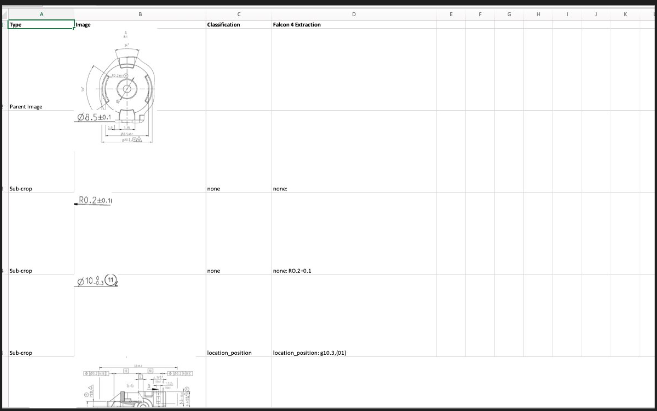
\includegraphics[width=\textwidth]{Excell.png}%
  \caption{Excel Sheet}
  \label{fig:Excel Sheet}
\end{figure}

\section{Deployment \& CI/CD Integration}
To ensure consistent runtime environments and seamless portability across development, testing, and production systems, the entire Falcon pipeline has been fully containerized using \textbf{Docker}. This guarantees that all dependencies, configurations, and versions remain uniform regardless of the host system, thus eliminating the common "it works on my machine" issue.

\subsection{Dockerization}

Each module within the pipeline—including preprocessing, sub-crop detection, classification, and data extraction—is encapsulated in its own Docker container. These modular containers interact via well-defined APIs and mounted volumes, enabling:

\begin{itemize}
    \item Clean separation of concerns
    \item Easier debugging and testing
    \item Reproducible experiments
    \item Simplified onboarding for new developers
\end{itemize}

Docker images are versioned and tagged according to both commit hashes and semantic versioning principles, enabling robust traceability and rollback capabilities.

\subsection{Automated Build \& Continuous Deployment via GitLab CI/CD}

A fully automated CI/CD pipeline is implemented using \textbf{GitLab CI} to streamline the development lifecycle. The workflow includes:

\begin{itemize}
    \item \textbf{Build Trigger:} Every commit or merge request to the main branch triggers a CI job.
    \item \textbf{Image Build:} A fresh Docker image is constructed using a predefined \texttt{Dockerfile}, incorporating the latest source code, environment variables, and dependencies.
    \item \textbf{Image Push:} The newly built image is pushed to a secured Docker container registry (self-hosted or GitLab container registry).
    \item \textbf{Automated Deployment:}
    \begin{itemize}
        \item The university’s server infrastructure, configured with secure access tokens, continuously polls for the latest Docker image.
        \item Upon detecting an updated image, the server automatically pulls and deploys it, ensuring that the most current version of the pipeline—including model weights, configurations, and scripts—is always live.
    \end{itemize}
\end{itemize}

This pipeline reduces downtime, enforces consistency, and accelerates the release cycle without requiring manual intervention.

\subsection{Scalability and Future-Proofing}

The pipeline is designed with extensibility and scalability in mind. Future enhancements are accommodated by the following architectural provisions:

\begin{itemize}
    \item \textbf{Support for LLM-Based Modules:} The system is prepared to integrate large language models (LLMs) for context-aware extraction and interpretation tasks, enabling semantic document understanding in downstream stages.
    \item \textbf{Vision Transformer (ViT) Compatibility:} The modular detection and classification stages support plug-and-play integration with transformer-based vision models, allowing the system to evolve with advancements in computer vision.
    \item \textbf{Agent-Based Resource Orchestration:} For high-load environments or cloud-scale deployment, the architecture supports agent-based orchestration (e.g., using Kubernetes or Nomad). These agents can dynamically allocate and scale compute resources, enabling parallel job execution, load balancing, and fault tolerance.
\end{itemize}


\section{Next Steps}
With a foundational solution in place and positive initial results, the project will now move into subsequent phases to enhance and expand the system. The next steps include:

\begin{enumerate}
  \item \textbf{Incorporating Real Drawing Data:} We will gather a set of actual engineering drawings from PSM Protech (or similar sources) and create a ground-truth dataset of tolerance annotations. This may involve manually labeling some drawings to identify tolerance symbol regions and their true values. We will then evaluate our current models on this data to identify gaps between synthetic and real performance.
  \item \textbf{Training Object Detection for Region Localization:} The current pipeline assumes the tolerance annotation images are given. The next development step is to train an object detection model (likely using YOLOv8 in detection mode) to automatically find tolerance feature control frames and related text in a full drawing. We will need to prepare training data for this, possibly by annotating bounding boxes on drawings around the tolerance frames. This detector will allow us to feed those cropped regions into the classifier and OCR modules, automating the region-of-interest extraction.
  \item \textbf{Expanding Tolerance Classes:} We plan to include more types of tolerances in the classification model. For example, adding classes for perpendicularity, parallelism, position, etc. This will require sourcing or synthesizing images of those symbols and retraining or fine-tuning the classification model. The YOLO model can be fine-tuned on new classes with relatively small additional data.
  \item \textbf{Improving OCR and Data Parsing:} For more complex annotations, we may need to capture additional information. For instance, a position tolerance has a number and datum references (e.g., $\varphi 0.2 \textbf{A}\textbf{B}\textbf{C}$). Our current OCR is only extracting “0.2”. We might improve this by either a specialized parser or by running OCR in a mode that also captures letters and then interpreting those letters (e.g., they are datums or material condition symbols). We will also investigate if using Tesseract’s layout analysis or other OCR engines yields better results for small text.
  \item \textbf{User Interface and Visualization:} As the backend becomes more capable, we will consider developing a simple user interface to visualize the results. This could be a tool that a user loads a drawing into and sees highlighted tolerance annotations with their interpreted values and types. Even a command-line interface or a Jupyter notebook demonstration could be useful for internal presentations and getting feedback.
  \item \textbf{Performance Optimization:} We will profile the pipeline on larger inputs and optimize where necessary. For example, if converting images to PDF and back is too slow for dozens of annotations, we might streamline that or use an alternative approach (like direct image segmentation for columns without PDF conversion).
  \item \textbf{Continuous Model Improvement:} Based on errors observed on new data, we will refine our models. This could mean more training data, adjusting hyperparameters, or even trying different model architectures if needed. For the OCR part, if certain digits or formats are consistently misread, we might implement post-processing rules (for example, if we know all tolerances are under 1.0, then an OCR result of “10” might actually be “0.0” misread).
  \item \textbf{Documentation and Knowledge Sharing:} We will keep this document up-to-date with new findings and system changes. Additionally, we plan to write a user guide for the end system and a developer guide for future maintainers. As the project continues, more team members (such as student assistants or new hires) might join, and comprehensive documentation will be crucial for onboarding them efficiently.
\end{enumerate}

By following these next steps, we aim to transition from a feasibility demo to a more robust prototype. The ultimate vision is a system integrated into PSM Protech’s workflow, where an engineer can upload a drawing and receive an automated report highlighting tolerance information. Each step above brings us closer to that goal: improving accuracy, broadening scope, and ensuring the solution is practical in a real-world setting.

\section{Quality Assurance Test Results}

This chapter provides an overview of the quality assurance testing conducted to evaluate the effectiveness of the developed models. Testing was performed on two different blueprints provided by the customer, on which the models were initially trained.

\subsection{Category 1: Big Crop Model (Gear Drawings)}
\begin{itemize}
  \item \textbf{Sheet 1:} 7 out of 14 crops were successfully automatically cropped by the model.
  \item \textbf{Sheet 2:} 4 out of 5 crops were successfully automatically cropped by the model.
\end{itemize}

\subsection{Category 2: Small Crop Model (Rectangle Shapes)}
\begin{itemize}
  \item \textbf{Sheet 1:} 31 out of 55 crops were successfully automatically cropped by the model.
  \item \textbf{Sheet 2:} 26 out of 32 crops were successfully automatically cropped by the model.
\end{itemize}

\subsection{Category 3: Classification Model}
\begin{itemize}
  \item Most symbols were classified as \textbf{None}, as no relevant symbols were present for extraction.
  \item The model exhibited a bias toward the \textbf{Location (Position)} class.
\end{itemize}

\subsection{Category 4: OCR Extraction Model}
\begin{table}[h!]
\centering
\begin{tabular}{|l|c|c|}
\hline
\textbf{Evaluation Level} & \textbf{Sheet 1 Results} & \textbf{Sheet 2 Results} \\
\hline
Best & 1 out of 30 & 3 out of 46 \\
\hline
Good & 8 out of 31 & 13 out of 46 \\
\hline
Hallucinations/None & 19 out of 31 & 30 out of 46 \\
\hline
\end{tabular}
\caption{OCR Extraction Model Evaluation}
\end{table}

\subsection*{Summary}
The conducted quality assurance tests demonstrate the varying performance of each model category. Notably, the cropping models performed reliably for specific shapes, with significant performance variations influenced by the number of gear drawings per blueprint. Specifically, Sheet 2 had fewer gear drawings than Sheet 1, which resulted in noticeably better cropping accuracy for both big and small crop models. This observation indicates that the density of gear drawings per blueprint directly influences the model's general cropping accuracy. Conversely, OCR extraction displayed a higher rate of misclassifications or omissions, highlighting the necessity for targeted improvements in this area. These insights will guide future enhancements and training to further optimize model accuracy and reliability.

Regarding the results of the classification model, most outputs were categorized as the 	extbf{None} class. This behavior can be explained by the fact that several symbols present in the test data were not included in the original training set. Furthermore, when classification did occur, it was predominantly into the 	extbf{Location (Position)} class. This trend indicates a clear model bias, likely stemming from an overrepresentation of this class in the training data.

To mitigate this issue, the training dataset must be expanded to include a broader variety of symbol classes. A more diverse dataset would help balance class representation and improve the model’s ability to generalize, thereby reducing the tendency to default to a dominant class such as 	extit{Location (Position)}.

\section*{Analysis of Results}

The number of gear drawings per blueprint substantially affects model performance. Sheet 2, containing fewer gear drawings, demonstrated higher accuracy in cropping compared to Sheet 1. This suggests a correlation between the complexity and density of gear drawings and the model’s accuracy, which should be considered in future model training and blueprint selection to maximize efficiency and accuracy.

\section{Conclusion}
In this feasibility study, we demonstrated the potential of a hybrid computer vision approach to automate the reading of geometric tolerances from engineering drawings. Through the use of a tolerance classification model and an OCR extraction pipeline, the system can interpret simplified representations of tolerance callouts. The project has laid the groundwork with synthetic data and initial models, and the results so far are encouraging. Moving forward, the focus will be on scaling up the solution to handle real drawings, more tolerance types, and integrating all components seamlessly. With continued development, this project could significantly streamline the feasibility analysis of designs at PSM Protech, saving time and reducing errors in the engineering process.


\begin{thebibliography}{9}
\begin{itemize}
  \item A. Zheng, B. Smith, and C. Lee, “Hybrid Deep-Learning for Structured Extraction from Engineering Drawings,” \textit{Proceedings of the International Conference on Document Analysis and Recognition}, 2025.
  \item B. Xu, D. Kumar, and E. Chen, “Tolerance Information Extraction from Mechanical Drawings using CNNs,” \textit{Journal of Computational Engineering}, vol. 12, no. 3, pp. 45–58, 2024.
  \item F. Garcia et al., “eDOCr2: Enhanced Document OCR and Retrieval,” \textit{MDPI Journal of Data Science}, vol. 8, 2023.
  \item M. Bakkopi, “engineering-drawing-extractor,” \texttt{https://github.com/bakkopi/engineering-drawing-extractor}, accessed May 2025.
  \item Werk24 API Documentation, \url{https://werk24.com/api/docs}, accessed May 2025.
  \item Infrrd AI Services, \url{https://www.infrrd.ai/services}, accessed May 2025.
  \item Markovate AI Blueprint Reader, \url{https://www.markovate.com/blueprint-reader}, accessed May 2025.
\end{itemize}
\end{thebibliography}

\vfill
\begin{center}
*** End of Document ***
\end{center}

\end{document}

